\documentclass{beamer}

\newenvironment{tightcenter}{%
  \setlength\topsep{0pt}
  \setlength\parskip{0pt}
  \begin{center}
}{%
  \end{center}
}

\mode<presentation>
{
  \usetheme{Copenhagen}
  %%\usecolortheme[RGB={173,222,25}]{structure}
  \usecolortheme[RGB={255,0,0}]{structure}
  \setbeamertemplate{items}[circle]
  \setbeamercovered{transparent}
}

\usepackage[polish]{babel}
\usepackage{chessfss}
\usepackage{hyperref}
\usepackage{qtree}
\usepackage{mathtools}
\usepackage{dirtytalk}
\usepackage{epigraph}
\usepackage{textgreek}
\usepackage[utf8]{inputenc}
\usepackage{times}
\usepackage[T1]{fontenc}
\usepackage{tikz}
\usepackage{csquotes}
\usepackage{amsmath}
\usepackage{fancyvrb}
\usepackage{ulem}
\usepackage{adjustbox}

\newenvironment{Snippet}{\Verbatim[samepage=true]}{\endVerbatim}

\title{\textbf{Czym do diaska jest programowanie funkcyjne?}}

\author{Panicz Maciej Godek}

\institute{
  \tiny{\href{mailto:godek.maciek@gmail.com}{\textbf{godek.maciek@gmail.com}}}
}

\date{\textbf{Hackerspace Trójmiasto}, 07.02.2017}

\begin{document}

\begin{frame}
  \titlepage
\end{frame}

\section{Wprowadzenie}

\begin{frame}{Definicja}
  \textbf{Czym jest programowanie?}
  \pause
  \begin{itemize}
  \item stosunkowo młoda dziedzina ludzkiej działalności
    \pause
    \\ ale czy na pewno?
    \pause
    \begin{displayquote}
      ,,Nauczyciele, generałowie, dietetycy, psychologowie i rodzice programują.
      Działania wojska, studentów i niektórych społeczności są programowane.
      Zmierzenie się z dużym problemem wymaga wielu programów, z których
      większość jest powoływana do życia w trakcie tych zmagań.''
    \end{displayquote}
    -- Alan Perlis
    
  \end{itemize}

\end{frame}

\begin{frame}{Analogia}
  \textbf{Do jakiej innej dziedziny ludzkiej działalności
    można porównać programowanie?}
  \pause
  \begin{itemize}
  \item budowanie urządzeń\pause, które \\
    przeprowadzając kolejne kroki \\
    \pause zmieniają swój stan
    \pause
  \item logika, wyrażanie idei \\
    \pause (definicje, twierdzenia, dowody, przykłady)
  \end{itemize}
\end{frame}


\begin{frame}{Analogia}
  \textbf{Do jakiej innej dziedziny ludzkiej działalności
    można porównać programowanie?}
  \begin{itemize}
  \item budowanie urządzeń, które \\
    przeprowadzając kolejne kroki \\
    \sout{zmieniają swój stan}
  \item logika, wyrażanie idei \\
    (definicje, twierdzenia, dowody, przykłady)
  \end{itemize}
\end{frame}


\begin{frame}{Analogia}
  \textbf{Do jakiej innej dziedziny ludzkiej działalności
    można porównać programowanie?}
  \begin{itemize}
  \item budowanie urządzeń\sout{, które \\
    przeprowadzając kolejne kroki} \\
    \sout{zmieniają swój stan}
  \item logika, wyrażanie idei \\
    (definicje, twierdzenia, dowody, przykłady)
  \end{itemize}
\end{frame}


\begin{frame}{Analogia}
  \textbf{Do jakiej innej dziedziny ludzkiej działalności
    można porównać programowanie?}
  \begin{itemize}
  \item \sout{budowanie urządzeń}\sout{, które \\
      przeprowadzając kolejne kroki} \\
    \sout{zmieniają swój stan}
  \item logika, wyrażanie idei \\
    (definicje, twierdzenia, dowody, przykłady)
  \end{itemize}
\end{frame}

\section{Przykład}

\begin{frame}{Przykład}

  \textbf{Program, który liczy sumę kwadratów
    początkowych siedmiu liczb pierwszych}

  \pause
  \texttt{licznik := 7\\*
liczba := 0\\*
suma := 0\\*
dopóki(licznik > 0):\\*
\ \ \ \ jeżeli jest\_pierwsza(liczba):\\*
\ \ \ \ \ \ \ \ suma := suma + liczba\^{}2\\*
\ \ \ \ \ \ \ \ licznik := licznik - 1\\*
\ \ \ \ liczba := liczba + 1
  }
   
\end{frame}

\begin{frame}{Schemat blokowy}
  \begin{center}
    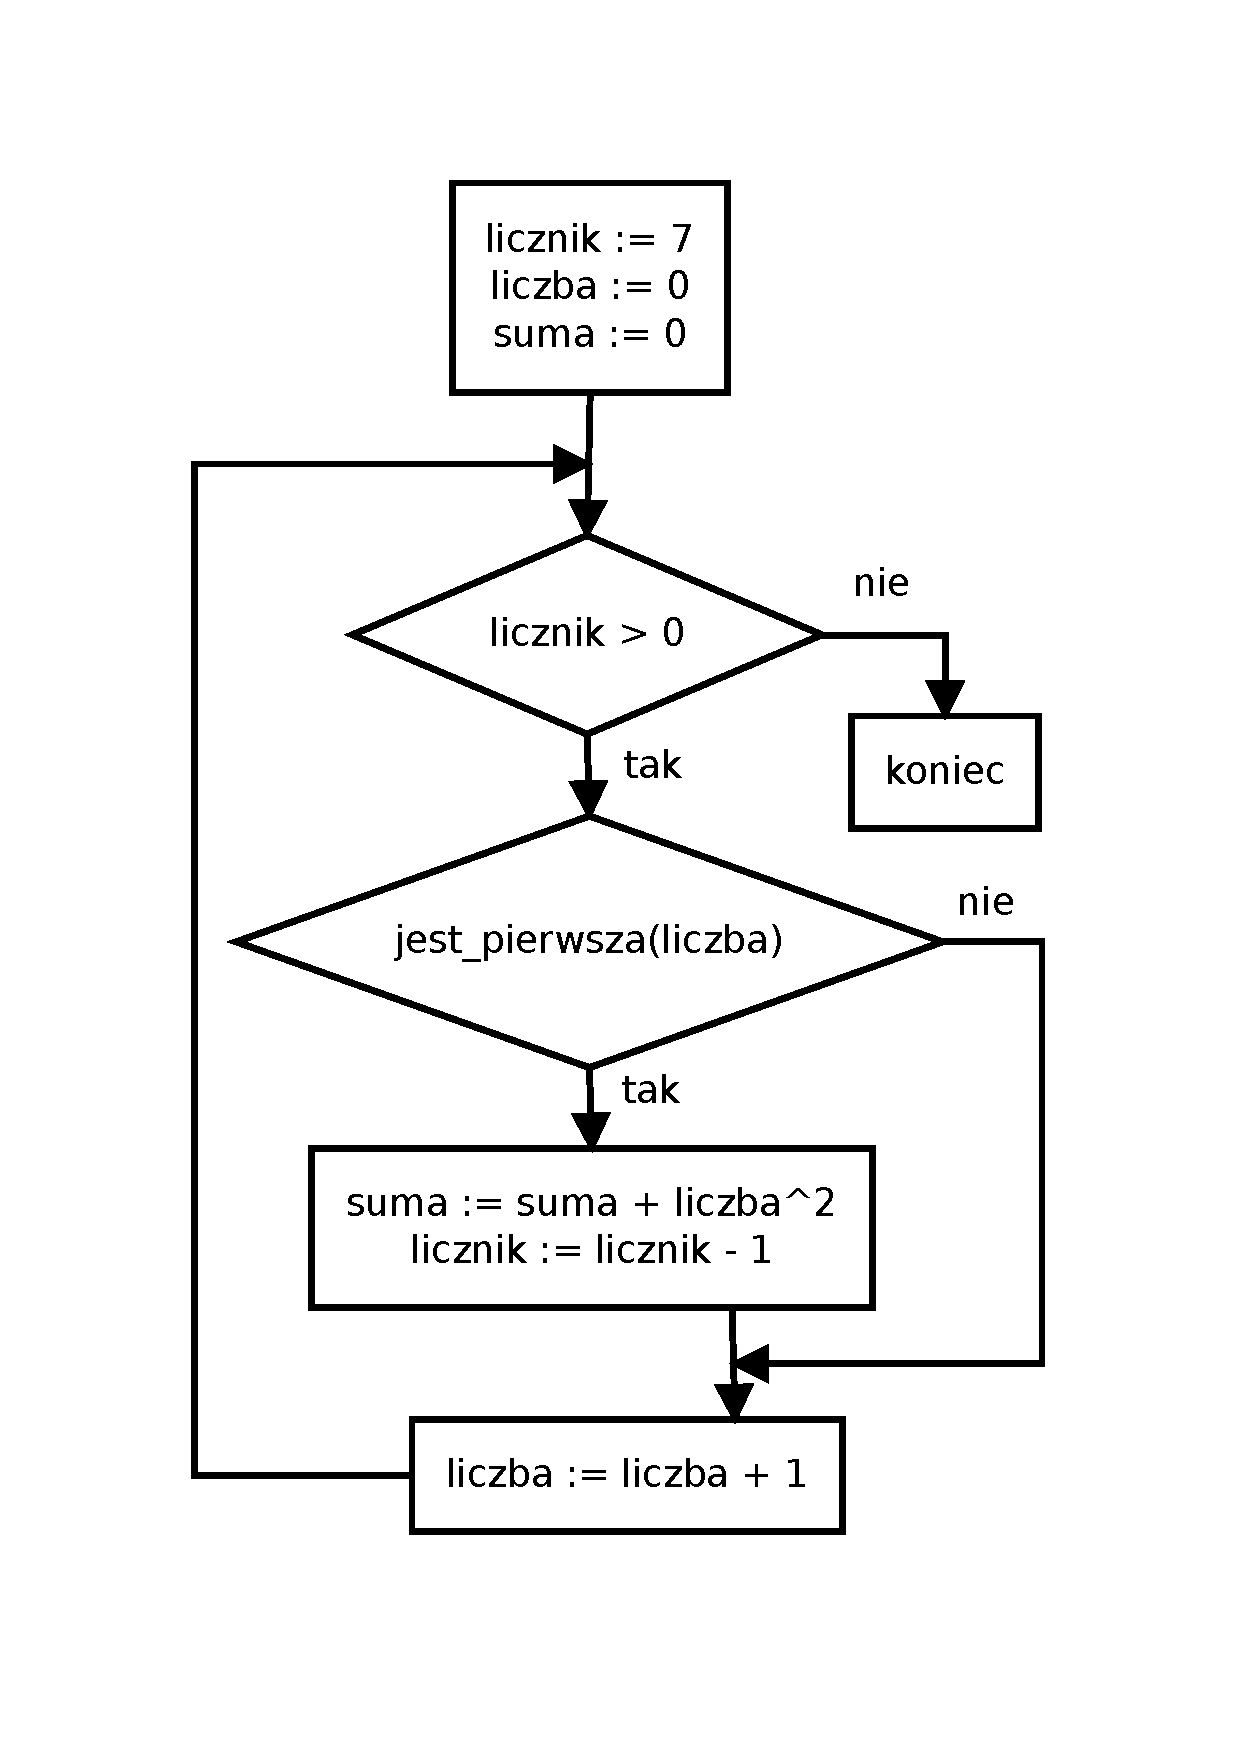
\includegraphics[width=\textwidth,height=0.8\textheight,keepaspectratio]{pierwsze.pdf}
  \end{center}
\end{frame}

\begin{frame}{Perspektywa lingwistyczna}
  \textbf{suma kwardatów początkowych siedmiu liczb pierwszych} \\
  \pause
  ,,suma $X$''\pause, gdzie \\
  $X$ = ,,kwardaty $Y$''\pause, gdzie \\
  $Y$ = ,,$k$ początkowych liczb pierwszych''\pause, gdzie \\
  $k$ = 7
\end{frame}

\begin{frame}{Drzewko}

  \begin{center}
    \Tree [.suma
      [.kwadratów
        [.liczb-pierwszych siedmiu początkowych ] ] ]
  \end{center}
  
\end{frame}

\begin{frame}
  ,,suma kwadratów początkowych siedmiu liczb pierwszych'' \\
  
  Do wyjaśnienia: \pause
  \begin{itemize}
  \item co znaczy ,,suma $X$''? \pause
  \item co znaczy ,,kwadraty $Y$'' \pause
  \item co znaczy ,,siedem początkowych liczb pierwszych''?
  \end{itemize}
\end{frame}

\begin{frame}{Znaczenie}
  \textbf{Co znaczy ,,siedem początkowych liczb pierwszych''?} \\
  \pause
  \begin{center}
    \begin{tabular}{ l c r }
      denotacja & vs. & konotacja \pause\\
    \end{tabular}
  \end{center}
  \begin{itemize}
  \item denotacja (odniesienie): obiekt, do którego dane wyrażenie językowe się
    \textit{odnosi}\pause, np. ciąg \texttt{(2 3 5 7 11 13 17)} \pause
  \item konotacja (określenie): inne wyrażenie językowe równoważne danemu
    (ale prostsze pojęciowo)
  \end{itemize}
  
\end{frame}

\begin{frame}{Redukcja}
  \textbf{Konotacja (definicja)}
 
  Niech $N$ i $M$ oznaczają liczby naturalne. Rozważmy znaczenie wyrażenia \\
  ,,$N$ najmniejszych liczb pierwszych większych od $M$'' \pause \\

  \begin{enumerate}
  \item wiemy, że znaczeniem tego wyrażenia (o ile jest sensowne)
    jest \textbf{ciąg} $N$-elementowy \pause
    
  \item znaczenie wyrażenia ,,$0$ najmniejszych liczb pierwszych
    większych od $M$'' jest \textbf{tożsame} (koekstensjonalne)
    ze znaczeniem wyrażenia ,,pusty ciąg''
  \end{enumerate}
    
\end{frame}

\begin{frame}{Redukcja}
  \textbf{Konotacja (definicja)} 
  Niech $N$ i $M$ oznaczają liczby naturalne. Rozważmy znaczenie wyrażenia \\
  ,,$N+1$ najmniejszych liczb pierwszych większych od $M$'' \pause \\

  \begin{enumerate}
    \setcounter{enumi}{2}
    \item jeżeli $M+1$ jest liczbą pierwszą, to znaczeniem wyrażenia
    ,,$N+1$ najmniejszych liczb pierwszych większych od $M$'' jest \textbf{ciąg},
    którego pierwszym elementem jest $M+1$, a którego pozostałe elementy
    to ,,$N$ najmniejszych liczb pierwszych większych od $M+1$ \pause
    
  \item jeżeli $M+1$ nie jest liczbą pierwszą, to znaczenie wyrażenia
    ,,$N+1$ najmniejszych liczb pierwszych większych od $M$'' jest
    \textbf{takie samo}, jak znaczenie wyrażenia ,,$N+1$ liczb pierwszych
    większych od $M+1$''.
  \end{enumerate}
\end{frame}

\begin{frame}
  \center{Uff...}
\end{frame}

\begin{frame}{Formalna notacja}

  \textbf{suma kwadratów początkowych siedmiu liczb pierwszych}
  \pause
  sum of squares of initial seven prime numbers 
  {\tiny (angielski nie ma deklinacji)} \\
  \pause
  \texttt{(sum (squares (initial seven prime numbers)))} {\tiny(złożone
    deskrypcje bierzemy w nawiasy, \texttt{f} of \texttt{x} = \texttt{(f x)})} \\
  \pause
  \textbf{\texttt{(sum (squares (prime-numbers seven initial)))}}
  {\tiny(słowa rządzące na początku)} \\

\end{frame}

\begin{frame}{Język Scheme}
  \texttt{
(define (prime-numbers amount lowest)\\*
\ \ (if (equal?\ amount 0)\\*
\ \ \ \ '()\\*
\ \ \ \ (if (prime?\ lowest)\\*
\ \ \ \ \ \ (cons lowest (prime-numbers (- amount 1)\\*
\ \ \ \ \ \ \ \ \ \ \ \ \ \ \ \ \
\ \ \ \ \ \ \ \ \ \ \ \ \ \ \ (+ lowest 1)))\\*
\ \ \ \ \ \ (prime-numbers amount (+ lowest 1)))))\\*
  }
\end{frame}

\begin{frame}{Język Scheme}
  \texttt{
(\textbf{define (prime-numbers amount lowest)}\\*
\ \ (if (equal?\ amount 0)\\*
\ \ \ \ '()\\*
\ \ \ \ (if (prime?\ lowest)\\*
\ \ \ \ \ \ (cons lowest (prime-numbers (- amount 1)\\*
\ \ \ \ \ \ \ \ \ \ \ \ \ \ \ \ \
\ \ \ \ \ \ \ \ \ \ \ \ \ \ \ (+ lowest 1)))\\*
\ \ \ \ \ \ (prime-numbers amount (+ lowest 1)))))\\*
  }
\end{frame}

\begin{frame}{Język Scheme}
  \texttt{
(define (prime-numbers amount lowest)\\*
\ \ \textbf{(if (equal?\ amount 0)\\*
\ \ \ \ '()\\*
\ \ \ \ (if (prime?\ lowest)\\*
\ \ \ \ \ \ (cons lowest (prime-numbers (- amount 1)\\*
\ \ \ \ \ \ \ \ \ \ \ \ \ \ \ \ \
\ \ \ \ \ \ \ \ \ \ \ \ \ \ \ (+ lowest 1)))\\*
\ \ \ \ \ \ (prime-numbers amount (+ lowest 1))))})\\*
  }
\end{frame}

\begin{frame}{Język Scheme}
  \texttt{
(define (prime-numbers amount lowest)\\*
\ \ (if \textbf{(equal?\ amount 0)\\*
\ \ \ \ '()}\\*
\ \ \ \ (if (prime?\ lowest)\\*
\ \ \ \ \ \ (cons lowest (prime-numbers (- amount 1)\\*
\ \ \ \ \ \ \ \ \ \ \ \ \ \ \ \ \
\ \ \ \ \ \ \ \ \ \ \ \ \ \ \ (+ lowest 1)))\\*
\ \ \ \ \ \ (prime-numbers amount (+ lowest 1)))))\\*
  }
\end{frame}


\begin{frame}{Język Scheme}
  \texttt{
(define (prime-numbers amount lowest)\\*
\ \ (if (equal?\ amount 0)\\*
\ \ \ \ '()\\*
\ \ \ \ \textbf{(if (prime?\ lowest)\\*
\ \ \ \ \ \ (cons lowest (prime-numbers (- amount 1)\\*
\ \ \ \ \ \ \ \ \ \ \ \ \ \ \ \ \
\ \ \ \ \ \ \ \ \ \ \ \ \ \ \ (+ lowest 1)))\\*
\ \ \ \ \ \ (prime-numbers amount (+ lowest 1)))}))\\*
  }
\end{frame}

\begin{frame}{Język Scheme}
  \texttt{
(define (prime-numbers amount lowest)\\*
\ \ (if (equal?\ amount 0)\\*
\ \ \ \ '()\\*
\ \ \ \ (if \textbf{(prime?\ lowest)\\*
\ \ \ \ \ \ (cons lowest (prime-numbers (- amount 1)\\*
\ \ \ \ \ \ \ \ \ \ \ \ \ \ \ \ \
\ \ \ \ \ \ \ \ \ \ \ \ \ \ \ (+ lowest 1)))}\\*
\ \ \ \ \ \ (prime-numbers amount (+ lowest 1)))))\\*
  }
\end{frame}

\begin{frame}{Język Scheme}
  \texttt{
(define (prime-numbers amount lowest)\\*
\ \ (if (equal?\ amount 0)\\*
\ \ \ \ '()\\*
\ \ \ \ (if (prime?\ lowest)\\*
\ \ \ \ \ \ (cons lowest (prime-numbers (- amount 1)\\*
\ \ \ \ \ \ \ \ \ \ \ \ \ \ \ \ \
\ \ \ \ \ \ \ \ \ \ \ \ \ \ \ (+ lowest 1)))\\*
\ \ \ \ \ \ \textbf{(prime-numbers amount (+ lowest 1))})))\\*
  }
\end{frame}


\begin{frame}{Pojęcia pierwotne}
  Użyte pojęcia pierwotne: \pause
  \begin{itemize}
  \item \texttt{(if <warunek> <wartość> <alternatywa>)} -- jeżeli
    \texttt{<warunek>} jest spełniony, znaczeniem całego wyrażenia jest
    \texttt{<wartość>}, a w przeciwnym razie jest nią \texttt{<alternatywa>}\pause
  \item \texttt{(equal? a b)} -- \texttt{a} i \texttt{b} są równe\pause
  \item \texttt{(+ a b)} -- suma \texttt{a} i \texttt{b}\pause
  \item \texttt{(- a b)} -- różnica \texttt{a} i \texttt{b}\pause
  \item \texttt{(cons element sequence)} -- sekwencja, której pierwszym
    elementem jest \texttt{element}, zaś pozostałe elementy to elementy
    sekwencji \texttt{sequence}\pause
  \item \texttt{'()} -- sekwencja pusta
  \end{itemize}
\end{frame}

\begin{frame}{Pojęcia wtórne}
  Użyte pojęcia wtórne:\pause
  \begin{itemize}
  \item \texttt{prime-numbers} -- ale to je właśnie definiujemy
    (rekurencyjnie) \pause
  \item \texttt{(prime?\ n)} -- test, czy \texttt{n} jest liczbą pierwszą
  \end{itemize}
\end{frame}

\begin{frame}{Pierwszość liczby}
  $n$ jest \textit{liczbą pierwszą}, jeśli jej jedyne podzielniki
  to $1$ oraz $n$\pause
  \texttt{
(define (prime?\ n)\\*
\ \ (equal? (divisors n) (list 1 n)))\\*
    }\pause
  pojęcia pierwotne:\pause
  \begin{itemize}
  \item \texttt{(list arg1 arg2 ...)} -- lista (sekwencja) zawierająca argumenty
    \texttt{arg1}, \texttt{arg2}, \texttt{...}\pause
  \end{itemize}
  pojęcia wtórne:\pause
  \begin{itemize}
  \item \texttt{(divisors n)} -- lista wszystkich podzielników liczby naturalnej
    \texttt{n}
  \end{itemize}
  
\end{frame}

\begin{frame}{Podzielniki liczby}
  Liczba $1 \le k \le n$ jest \emph{podzielnikiem} liczby $n$ wtedy i tylko wtedy,
  gdy reszta z dzielenia $n$ przez $k$ wynosi zero\\
  \texttt{
(define (divisors n)\\*
\ \ (define (divisors n k)\\*
\ \ \ \ (if (> k n)\\*
\ \ \ \ \ \ '()\\*
\ \ \ \ \ \ (if (equal?\ (remainder n k) 0)\\*
\ \ \ \ \ \ \ \ (cons k (divisors n (+ k 1)))\\*
\ \ \ \ \ \ \ \ (divisors n (+ k 1)))))\\*
\ \ (divisors n 1))
\ \\*
\ \\*
  }
\end{frame}

\begin{frame}{Podzielniki liczby}
  Liczba $1 \le k \le n$ jest podzielnikiem liczby $n$ wtedy i tylko wtedy,
  gdy reszta z dzielenia $n$ przez $k$ wynosi zero\\
  \texttt{
(define (divisors n)\\*
\ \ \textbf{(define (divisors n k)\\*
\ \ \ \ (if (> k n)\\*
\ \ \ \ \ \ '()\\*
\ \ \ \ \ \ (if (equal?\ (remainder n k) 0)\\*
\ \ \ \ \ \ \ \ (cons k (divisors n (+ k 1)))\\*
\ \ \ \ \ \ \ \ (divisors n (+ k 1)))))}\\*
\ \ (divisors n 1))
\ \\*
\ \\*
  }
\end{frame}

\begin{frame}{Podzielniki liczby}
  Liczba $1 \le k \le n$ jest podzielnikiem liczby $n$ wtedy i tylko wtedy,
  gdy reszta z dzielenia $n$ przez $k$ wynosi zero\\
  \texttt{
(define (divisors n)\\*
\ \ (define (divisors n k)\\*
\ \ \ \ (if \textbf{(> k n)\\*
\ \ \ \ \ \ '()}\\*
\ \ \ \ \ \ (if (equal?\ (remainder n k) 0)\\*
\ \ \ \ \ \ \ \ (cons k (divisors n (+ k 1)))\\*
\ \ \ \ \ \ \ \ (divisors n (+ k 1)))))\\*
\ \ (divisors n 1)
\ \\*
\ \\*
  }
\end{frame}

\begin{frame}{Podzielniki liczby}
  Liczba $1 \le k \le n$ jest podzielnikiem liczby $n$ wtedy i tylko wtedy,
  gdy reszta z dzielenia $n$ przez $k$ wynosi zero\\
  \texttt{
(define (divisors n)\\*
\ \ (define (divisors n k)\\*
\ \ \ \ (if (> k n)\\*
\ \ \ \ \ \ '()\\*
\ \ \ \ \ \ \textbf{(if (equal?\ (remainder n k) 0)\\*
\ \ \ \ \ \ \ \ (cons k (divisors n (+ k 1)))\\*
\ \ \ \ \ \ \ \ (divisors n (+ k 1)))}))\\*
\ \ (divisors n 1))
\ \\*
\ \\*
  }
\end{frame}

\begin{frame}{Podzielniki liczby}
  Liczba $1 \le k \le n$ jest podzielnikiem liczby $n$ wtedy i tylko wtedy,
  gdy reszta z dzielenia $n$ przez $k$ wynosi zero\\
  \texttt{
(define (divisors n)\\*
\ \ (define (divisors n k)\\*
\ \ \ \ (if (> k n)\\*
\ \ \ \ \ \ '()\\*
\ \ \ \ \ \ (if \textbf{(equal?\ (remainder n k) 0)\\*
\ \ \ \ \ \ \ \ (cons k (divisors n (+ k 1)))}\\*
\ \ \ \ \ \ \ \ (divisors n (+ k 1)))))\\*
\ \ (divisors n 1))
\ \\*
\ \\*
  }
\end{frame}

\begin{frame}{Podzielniki liczby}
  Liczba $1 \le k \le n$ jest podzielnikiem liczby $n$ wtedy i tylko wtedy,
  gdy reszta z dzielenia $n$ przez $k$ wynosi zero\\
  \texttt{
(define (divisors n)\\*
\ \ (define (divisors n k)\\*
\ \ \ \ (if (> k n)\\*
\ \ \ \ \ \ '()\\*
\ \ \ \ \ \ (if (equal?\ (remainder n k) 0)\\*
\ \ \ \ \ \ \ \ (cons k (divisors n (+ k 1)))\\*
\ \ \ \ \ \ \ \ \textbf{(divisors n (+ k 1))})))\\*
\ \ (divisors n 1))
\ \\*
\ \\*
  }
\end{frame}

\begin{frame}{Podzielniki liczby}
  Liczba $1 \le k \le n$ jest podzielnikiem liczby $n$ wtedy i tylko wtedy,
  gdy reszta z dzielenia $n$ przez $k$ wynosi zero\\
  \texttt{
(define (divisors n)\\*
\ \ (define (divisors n k)\\*
\ \ \ \ (if (> k n)\\*
\ \ \ \ \ \ '()\\*
\ \ \ \ \ \ (if (equal?\ (remainder n k) 0)\\*
\ \ \ \ \ \ \ \ (cons k (divisors n (+ k 1)))\\*
\ \ \ \ \ \ \ \ (divisors n (+ k 1)))))\\*
\ \ \textbf{(divisors n 1)})
\ \\*
\ \\*
  }
\end{frame}

\begin{frame}{Analiza}
  Rozważmy \texttt{(divisors 4)}. Na mocy definicji mamy\pause\\
  \texttt{(divisors 4 1)}\pause\\
  \texttt{
(if (> 1 4)\\*
\ \ '()\\*
\ \ (if (equal?\ (remainder 4 1) 0)\\*
\ \ \ \ (cons 1 (divisors 4 (+ 1 1)))\\*
\ \ \ \ (divisors 4 (+ 1 1))))\\*
\ \\*
\ \\*
}
\end{frame}


\begin{frame}{Analiza}
  Rozważmy \texttt{(divisors 4)}. Na mocy definicji mamy\\
  \texttt{(divisors 4 1)}\\
  \texttt{
(if \textbf{(> 1 4)}\\*
\ \ '()\\*
\ \ (if (equal?\ (remainder 4 1) 0)\\*
\ \ \ \ (cons 1 (divisors 4 (+ 1 1)))\\*
\ \ \ \ (divisors 4 (+ 1 1))))\\*
\ \\*
\ \\*
}
\end{frame}

\begin{frame}{Analiza}
  Rozważmy \texttt{(divisors 4)}. Na mocy definicji mamy\\
  \texttt{(divisors 4 1)}\\
  \texttt{
(if \#false\\*
\ \ '()\\*
\ \ \textbf{(if (equal?\ (remainder 4 1) 0)\\*
\ \ \ \ (cons 1 (divisors 4 (+ 1 1)))\\*
\ \ \ \ (divisors 4 (+ 1 1)))})\\*
\ \\*
\ \\*
}
\end{frame}

\begin{frame}{Analiza}
  Rozważmy \texttt{(divisors 4)}. Na mocy definicji mamy\\
  \texttt{(divisors 4 1)}\\
  \texttt{
\textbf{(if (equal?\ (remainder 4 1) 0)\\*
\ \ (cons 1 (divisors 4 (+ 1 1)))\\*
\ \ (divisors 4 (+ 1 1)))}\\*
\ \\*
\ \\*
\ \\*
\ \\*
}
\end{frame}

\begin{frame}{Analiza}
  Rozważmy \texttt{(divisors 4)}. Na mocy definicji mamy\\
  \texttt{(divisors 4 1)}\\
  \texttt{
(if \textbf{(equal?\ (remainder 4 1) 0)}\\*
\ \ (cons 1 (divisors 4 (+ 1 1)))\\*
\ \ (divisors 4 (+ 1 1)))\\*
\ \\*
\ \\*
\ \\*
\ \\*
}
\end{frame}

\begin{frame}{Analiza}
  Rozważmy \texttt{(divisors 4)}. Na mocy definicji mamy\\
  \texttt{(divisors 4 1)}\\
  \texttt{
(if (equal?\ \textbf{(remainder 4 1)} 0)\\*
\ \ (cons 1 (divisors 4 (+ 1 1)))\\*
\ \ (divisors 4 (+ 1 1)))\\*
\ \\*
\ \\*
\ \\*
\ \\*
}
\end{frame}

\begin{frame}{Analiza}
  Rozważmy \texttt{(divisors 4)}. Na mocy definicji mamy\\
  \texttt{(divisors 4 1)}\\
  \texttt{
(if (equal?\ \textbf{0} 0)\\*
\ \ (cons 1 (divisors 4 (+ 1 1)))\\*
\ \ (divisors 4 (+ 1 1)))\\*
\ \\*
\ \\*
\ \\*
\ \\*
}
\end{frame}

\begin{frame}{Analiza}
  Rozważmy \texttt{(divisors 4)}. Na mocy definicji mamy\\
  \texttt{(divisors 4 1)}\\
  \texttt{
(if \textbf{(equal?\ 0 0)}\\*
\ \ (cons 1 (divisors 4 (+ 1 1)))\\*
\ \ (divisors 4 (+ 1 1)))\\*
\ \\*
\ \\*
\ \\*
\ \\*
}
\end{frame}

\begin{frame}{Analiza}
  Rozważmy \texttt{(divisors 4)}. Na mocy definicji mamy\\
  \texttt{(divisors 4 1)}\\
  \texttt{
(if \#true\\*
\ \ \textbf{(cons 1 (divisors 4 (+ 1 1)))}\\*
\ \ (divisors 4 (+ 1 1)))\\*
\ \\*
\ \\*
\ \\*
\ \\*
}
\end{frame}


\begin{frame}{Analiza}
  Rozważmy \texttt{(divisors 4)}. Na mocy definicji mamy\\
  \texttt{(divisors 4 1)}\\
  \texttt{
(cons 1 \textbf{(divisors 4 (+ 1 1))})\\*
\ \\*    
\ \\*
\ \\*
\ \\*
\ \\*
\ \\*
  }
\end{frame}

\begin{frame}{Analiza}
  Rozważmy \texttt{(divisors 4)}. Na mocy definicji mamy\\
  \texttt{(divisors 4 1)}\\
  \texttt{
(cons 1 (divisors 4 \textbf{(+ 1 1)}))\\*
\ \\*    
\ \\*
\ \\*
\ \\*
\ \\*
\ \\*
  }
\end{frame}

\begin{frame}{Analiza}
  Rozważmy \texttt{(divisors 4)}. Na mocy definicji mamy\\
  \texttt{(divisors 4 1)}\\
  \texttt{
(cons 1 (divisors 4 \textbf{2}))\\*
\ \\*    
\ \\*
\ \\*
\ \\*
\ \\*
\ \\*
  }
\end{frame}

\begin{frame}{Analiza}
  Rozważmy \texttt{(divisors 4)}. Na mocy definicji mamy\\
  \texttt{(divisors 4 1)}\\
  \texttt{
(cons 1 \textbf{(divisors 4 2)})\\*
\ \\*
\ \\*
\ \\*
\ \\*
\ \\*
\ \\*
  }
\end{frame}

\begin{frame}{Analiza}
  Rozważmy \texttt{(divisors 4)}. Na mocy definicji mamy\\
  \texttt{(divisors 4 1)}\\
  \texttt{
(cons 1 \textbf{(if (> 2 4)\\*
\ \ \ \ \ \ \ \ \ \ \ '()\\*
\ \ \ \ \ \ \ \ \ \ \ (if (equal?\ (remainder 4 2) 0)\\*
\ \ \ \ \ \ \ \ \ \ \ \ \ (cons 2 (divisors 4 (+ 2 1)))\\*
\ \ \ \ \ \ \ \ \ \ \ \ \ (divisors 4 (+ 2 1))))})
\ \\*
\ \\*
\ \\*
  }
\end{frame}


\begin{frame}{Analiza}
  Rozważmy \texttt{(divisors 4)}. Na mocy definicji mamy\\
  \texttt{(divisors 4 1)}\\
  \texttt{
(cons 1 (if \textbf{(> 2 4)}\\*
\ \ \ \ \ \ \ \ \ \ \ '()\\*
\ \ \ \ \ \ \ \ \ \ \ (if (equal?\ (remainder 4 2) 0)\\*
\ \ \ \ \ \ \ \ \ \ \ \ \ (cons 2 (divisors 4 (+ 2 1)))\\*
\ \ \ \ \ \ \ \ \ \ \ \ \ (divisors 4 (+ 2 1)))))
\ \\*
\ \\*
\ \\*
  }
\end{frame}

\begin{frame}{Analiza}
  Rozważmy \texttt{(divisors 4)}. Na mocy definicji mamy\\
  \texttt{(divisors 4 1)}\\
  \texttt{
(cons 1 (if \#false\\*
\ \ \ \ \ \ \ \ \ \ \ '()\\*
\ \ \ \ \ \ \ \ \ \ \ \textbf{(if (equal?\ (remainder 4 2) 0)\\*
\ \ \ \ \ \ \ \ \ \ \ \ \ (cons 2 (divisors 4 (+ 2 1)))\\*
\ \ \ \ \ \ \ \ \ \ \ \ \ (divisors 4 (+ 2 1)))}))
\ \\*
\ \\*
\ \\*
  }
\end{frame}

\begin{frame}{Analiza}
  Rozważmy \texttt{(divisors 4)}. Na mocy definicji mamy\\
  \texttt{(divisors 4 1)}\\
  \texttt{
(cons 1 \textbf{(if (equal?\ (remainder 4 2) 0)\\*
\ \ \ \ \ \ \ \ \ \ \ (cons 2 (divisors 4 (+ 2 1)))\\*
\ \ \ \ \ \ \ \ \ \ \ (divisors 4 (+ 2 1)))})\\*
    \ \\*
    \ \\*
    \ \\*
    \ \\*
  }
\end{frame}

\begin{frame}{Analiza}
  Rozważmy \texttt{(divisors 4)}. Na mocy definicji mamy\\
  \texttt{(divisors 4 1)}\\
  \texttt{
(cons 1 (if \textbf{(equal?\ (remainder 4 2) 0)}\\*
\ \ \ \ \ \ \ \ \ \ \ (cons 2 (divisors 4 (+ 2 1)))\\*
\ \ \ \ \ \ \ \ \ \ \ (divisors 4 (+ 2 1))))\\*
    \ \\*
    \ \\*
    \ \\*
    \ \\*
  }
\end{frame}

\begin{frame}{Analiza}
  Rozważmy \texttt{(divisors 4)}. Na mocy definicji mamy\\
  \texttt{(divisors 4 1)}\\
  \texttt{
(cons 1 (if (equal?\ \textbf{(remainder 4 2)} 0)\\*
\ \ \ \ \ \ \ \ \ \ \ (cons 2 (divisors 4 (+ 2 1)))\\*
\ \ \ \ \ \ \ \ \ \ \ (divisors 4 (+ 2 1))))\\*
    \ \\*
    \ \\*
    \ \\*
    \ \\*
  }
\end{frame}

\begin{frame}{Analiza}
  Rozważmy \texttt{(divisors 4)}. Na mocy definicji mamy\\
  \texttt{(divisors 4 1)}\\
  \texttt{
(cons 1 (if (equal?\ \textbf{0} 0)\\*
\ \ \ \ \ \ \ \ \ \ \ (cons 2 (divisors 4 (+ 2 1)))\\*
\ \ \ \ \ \ \ \ \ \ \ (divisors 4 (+ 2 1))))\\*
    \ \\*
    \ \\*
    \ \\*
    \ \\*
  }
\end{frame}

\begin{frame}{Analiza}
  Rozważmy \texttt{(divisors 4)}. Na mocy definicji mamy\\
  \texttt{(divisors 4 1)}\\
  \texttt{
(cons 1 (if \textbf{(equal?\ 0 0)}\\*
\ \ \ \ \ \ \ \ \ \ \ (cons 2 (divisors 4 (+ 2 1)))\\*
\ \ \ \ \ \ \ \ \ \ \ (divisors 4 (+ 2 1))))\\*
    \ \\*
    \ \\*
    \ \\*
    \ \\*
  }
\end{frame}

\begin{frame}{Analiza}
  Rozważmy \texttt{(divisors 4)}. Na mocy definicji mamy\\
  \texttt{(divisors 4 1)}\\
  \texttt{
(cons 1 (if \#true\\*
\ \ \ \ \ \ \ \ \ \ \ \textbf{(cons 2 (divisors 4 (+ 2 1)))}\\*
\ \ \ \ \ \ \ \ \ \ \ (divisors 4 (+ 2 1))))\\*
    \ \\*
    \ \\*
    \ \\*
    \ \\*
  }
\end{frame}

\begin{frame}{Analiza}
  Rozważmy \texttt{(divisors 4)}. Na mocy definicji mamy\\
  \texttt{(divisors 4 1)}\\
  \texttt{
(cons 1 \textbf{(cons 2 (divisors 4 (+ 2 1)))})\\*
    \ \\*
    \ \\*
    \ \\*
    \ \\*
    \ \\*
    \ \\*
  }
\end{frame}


\begin{frame}{Analiza}
  Rozważmy \texttt{(divisors 4)}. Na mocy definicji mamy\\
  \texttt{(divisors 4 1)}\\
  \texttt{
(cons 1 (cons 2 (divisors 4 \textbf{(+ 2 1)})))\\*
    \ \\*
    \ \\*
    \ \\*
    \ \\*
    \ \\*
    \ \\*
  }
\end{frame}

\begin{frame}{Analiza}
  Rozważmy \texttt{(divisors 4)}. Na mocy definicji mamy\\
  \texttt{(divisors 4 1)}\\
  \texttt{
(cons 1 (cons 2 (divisors 4 \textbf{3})))\\*
    \ \\*
    \ \\*
    \ \\*
    \ \\*
    \ \\*
    \ \\*
  }
\end{frame}

\begin{frame}{Analiza}
  Rozważmy \texttt{(divisors 4)}. Na mocy definicji mamy\\
  \texttt{(divisors 4 1)}\\
  \texttt{
(cons 1 \\*
\ \ (cons 2 \\*
\ \ \ \ \textbf{(divisors 4 3)}))\\*
    \ \\*
    \ \\*
    \ \\*
    \ \\*
  }
\end{frame}

\begin{frame}{Analiza}
  Rozważmy \texttt{(divisors 4)}. Na mocy definicji mamy\\
  \texttt{(divisors 4 1)}\\
  \texttt{
(cons 1 \\*
\ \ (cons 2 \\*
\ \ \ \ \textbf{(if (> 3 4)\\*
\ \ \ \ \ \ '()\\*
\ \ \ \ \ \ (if (equal?\ (remainder 4 3) 0)\\*
\ \ \ \ \ \ \ \ (cons 3 (divisors 4 (+ 4 1)))\\*
\ \ \ \ \ \ \ \ (divisors 4 (+ 3 1))))}))\\*
  }
\end{frame}

\begin{frame}{Analiza}
  Rozważmy \texttt{(divisors 4)}. Na mocy definicji mamy\\
  \texttt{(divisors 4 1)}\\
  \texttt{
(cons 1 \\*
\ \ (cons 2 \\*
\ \ \ \ (if \textbf{(> 3 4)}\\*
\ \ \ \ \ \ '()\\*
\ \ \ \ \ \ (if (equal?\ (remainder 4 3) 0)\\*
\ \ \ \ \ \ \ \ (cons 3 (divisors 4 (+ 4 1)))\\*
\ \ \ \ \ \ \ \ (divisors 4 (+ 3 1))))))\\*
  }
\end{frame}


\begin{frame}{Analiza}
  Rozważmy \texttt{(divisors 4)}. Na mocy definicji mamy\\
  \texttt{(divisors 4 1)}\\
  \texttt{
(cons 1 \\*
\ \ (cons 2 \\*
\ \ \ \ (if \#false\\*
\ \ \ \ \ \ '()\\*
\ \ \ \ \ \ \textbf{(if (equal?\ (remainder 4 3) 0)\\*
\ \ \ \ \ \ \ \ (cons 3 (divisors 4 (+ 4 1)))\\*
\ \ \ \ \ \ \ \ (divisors 4 (+ 3 1)))})))\\*
  }
\end{frame}


\begin{frame}{Analiza}
  Rozważmy \texttt{(divisors 4)}. Na mocy definicji mamy\\
  \texttt{(divisors 4 1)}\\
  \texttt{
(cons 1 \\*
\ \ (cons 2 \\*
\ \ \ \ \textbf{(if (equal?\ (remainder 4 3) 0)\\*
\ \ \ \ \ \ (cons 3 (divisors 4 (+ 4 1)))\\*
\ \ \ \ \ \ (divisors 4 (+ 3 1)))}))\\*
\ \\*
\ \\*
  }
\end{frame}

\begin{frame}{Analiza}
  Rozważmy \texttt{(divisors 4)}. Na mocy definicji mamy\\
  \texttt{(divisors 4 1)}\\
  \texttt{
(cons 1 \\*
\ \ (cons 2 \\*
\ \ \ \ (if \textbf{(equal?\ (remainder 4 3) 0)}\\*
\ \ \ \ \ \ (cons 3 (divisors 4 (+ 4 1)))\\*
\ \ \ \ \ \ (divisors 4 (+ 3 1)))))\\*
\ \\*
\ \\*
  }
\end{frame}

\begin{frame}{Analiza}
  Rozważmy \texttt{(divisors 4)}. Na mocy definicji mamy\\
  \texttt{(divisors 4 1)}\\
  \texttt{
(cons 1 \\*
\ \ (cons 2 \\*
\ \ \ \ (if \textbf{(equal?\ (remainder 4 3) 0)}\\*
\ \ \ \ \ \ (cons 3 (divisors 4 (+ 4 1)))\\*
\ \ \ \ \ \ (divisors 4 (+ 3 1)))))\\*
\ \\*
\ \\*
  }
\end{frame}

\begin{frame}{Analiza}
  Rozważmy \texttt{(divisors 4)}. Na mocy definicji mamy\\
  \texttt{(divisors 4 1)}\\
  \texttt{
(cons 1 \\*
\ \ (cons 2 \\*
\ \ \ \ (if (equal?\ \textbf{(remainder 4 3)} 0)\\*
\ \ \ \ \ \ (cons 3 (divisors 4 (+ 4 1)))\\*
\ \ \ \ \ \ (divisors 4 (+ 3 1)))))\\*
\ \\*
\ \\*
  }
\end{frame}


\begin{frame}{Analiza}
  Rozważmy \texttt{(divisors 4)}. Na mocy definicji mamy\\
  \texttt{(divisors 4 1)}\\
  \texttt{
(cons 1 \\*
\ \ (cons 2 \\*
\ \ \ \ (if (equal?\ \textbf{1} 0)\\*
\ \ \ \ \ \ (cons 3 (divisors 4 (+ 4 1)))\\*
\ \ \ \ \ \ (divisors 4 (+ 3 1)))))\\*
\ \\*
\ \\*
  }
\end{frame}


\begin{frame}{Analiza}
  Rozważmy \texttt{(divisors 4)}. Na mocy definicji mamy\\
  \texttt{(divisors 4 1)}\\
  \texttt{
(cons 1 \\*
\ \ (cons 2 \\*
\ \ \ \ (if \texttt{(equal?\ 1 0)}\\*
\ \ \ \ \ \ (cons 3 (divisors 4 (+ 4 1)))\\*
\ \ \ \ \ \ (divisors 4 (+ 3 1)))))\\*
\ \\*
\ \\*
  }
\end{frame}

\begin{frame}{Analiza}
  Rozważmy \texttt{(divisors 4)}. Na mocy definicji mamy\\
  \texttt{(divisors 4 1)}\\
  \texttt{
(cons 1 \\*
\ \ (cons 2 \\*
\ \ \ \ (if \#false\\*
\ \ \ \ \ \ (cons 3 (divisors 4 (+ 4 1)))\\*
\ \ \ \ \ \ \textbf{(divisors 4 (+ 3 1))})))\\*
\ \\*
\ \\*
  }
\end{frame}

\begin{frame}{Analiza}
  Rozważmy \texttt{(divisors 4)}. Na mocy definicji mamy\\
  \texttt{(divisors 4 1)}\\
  \texttt{
(cons 1 \\*
\ \ (cons 2 \\*
\ \ \ \ \textbf{(divisors 4 (+ 3 1))}))\\*
\ \\*
\ \\*
\ \\*
\ \\*
  }
\end{frame}

\begin{frame}{Analiza}
  Rozważmy \texttt{(divisors 4)}. Na mocy definicji mamy\\
  \texttt{(divisors 4 1)}\\
  \texttt{
(cons 1 \\*
\ \ (cons 2 \\*
\ \ \ \ (divisors 4 \textbf{(+ 3 1)})))\\*
\ \\*
\ \\*
\ \\*
\ \\*
  }
\end{frame}

\begin{frame}{Analiza}
  Rozważmy \texttt{(divisors 4)}. Na mocy definicji mamy\\
  \texttt{(divisors 4 1)}\\
  \texttt{
(cons 1 \\*
\ \ (cons 2 \\*
\ \ \ \ (divisors 4 \textbf{4})))\\*
\ \\*
\ \\*
\ \\*
\ \\*
  }
\end{frame}

\begin{frame}{Analiza}
  Rozważmy \texttt{(divisors 4)}. Na mocy definicji mamy\\
  \texttt{(divisors 4 1)}\\
  \texttt{
(cons 1 \\*
\ \ (cons 2 \\*
\ \ \ \ \textbf{(divisors 4 4)}))\\*
\ \\*
\ \\*
\ \\*
\ \\*
  }
\end{frame}


\begin{frame}{Analiza}
  Rozważmy \texttt{(divisors 4)}. Na mocy definicji mamy\\
  \texttt{(divisors 4 1)}\\
  \texttt{
(cons 1 \\*
\ \ (cons 2 \\*
\ \ \ \ \textbf{(if (> 4 4)\\*
\ \ \ \ \ \ '()\\*
\ \ \ \ \ \ (if (equal?\ (remainder 4 4) 0)\\*
\ \ \ \ \ \ \ \ (cons 4 (divisors 4 (+ 4 1)))\\*
\ \ \ \ \ \ \ \ (divisors 4 (+ 4 1))))}))\\*
  }
\end{frame}

\begin{frame}{Analiza}
  Rozważmy \texttt{(divisors 4)}. Na mocy definicji mamy\\
  \texttt{(divisors 4 1)}\\
  \texttt{
(cons 1 \\*
\ \ (cons 2 \\*
\ \ \ \ (if \textbf{(> 4 4)}\\*
\ \ \ \ \ \ '()\\*
\ \ \ \ \ \ (if (equal?\ (remainder 4 4) 0)\\*
\ \ \ \ \ \ \ \ (cons 4 (divisors 4 (+ 4 1)))\\*
\ \ \ \ \ \ \ \ (divisors 4 (+ 4 1))))))\\*
  }
\end{frame}

\begin{frame}{Analiza}
  Rozważmy \texttt{(divisors 4)}. Na mocy definicji mamy\\
  \texttt{(divisors 4 1)}\\
  \texttt{
(cons 1 \\*
\ \ (cons 2 \\*
\ \ \ \ (if \#false\\*
\ \ \ \ \ \ '()\\*
\ \ \ \ \ \ \textbf{(if (equal?\ (remainder 4 4) 0)\\*
\ \ \ \ \ \ \ \ (cons 4 (divisors 4 (+ 4 1)))\\*
\ \ \ \ \ \ \ \ (divisors 4 (+ 4 1)))})))\\*
  }
\end{frame}


\begin{frame}{Analiza}
  Rozważmy \texttt{(divisors 4)}. Na mocy definicji mamy\\
  \texttt{(divisors 4 1)}\\
  \texttt{
(cons 1 \\*
\ \ (cons 2 \\*
\ \ \ \ (if \textbf{(equal?\ (remainder 4 4) 0)}\\*
\ \ \ \ \ \ (cons 4 (divisors 4 (+ 4 1)))\\*
\ \ \ \ \ \ (divisors 4 (+ 4 1)))))\\*
\ \\*
\ \\*
  }
\end{frame}

\begin{frame}{Analiza}
  Rozważmy \texttt{(divisors 4)}. Na mocy definicji mamy\\
  \texttt{(divisors 4 1)}\\
  \texttt{
(cons 1 \\*
\ \ (cons 2 \\*
\ \ \ \ (if (equal?\ \textbf{(remainder 4 4)} 0)\\*
\ \ \ \ \ \ (cons 4 (divisors 4 (+ 4 1)))\\*
\ \ \ \ \ \ (divisors 4 (+ 4 1)))))\\*
\ \\*
\ \\*
  }
\end{frame}

\begin{frame}{Analiza}
  Rozważmy \texttt{(divisors 4)}. Na mocy definicji mamy\\
  \texttt{(divisors 4 1)}\\
  \texttt{
(cons 1 \\*
\ \ (cons 2 \\*
\ \ \ \ (if (equal?\ \textbf{0} 0)\\*
\ \ \ \ \ \ (cons 4 (divisors 4 (+ 4 1)))\\*
\ \ \ \ \ \ (divisors 4 (+ 4 1)))))\\*
\ \\*
\ \\*
  }
\end{frame}

\begin{frame}{Analiza}
  Rozważmy \texttt{(divisors 4)}. Na mocy definicji mamy\\
  \texttt{(divisors 4 1)}\\
  \texttt{
(cons 1 \\*
\ \ (cons 2 \\*
\ \ \ \ (if \textbf{(equal?\ 0 0)}\\*
\ \ \ \ \ \ (cons 4 (divisors 4 (+ 4 1)))\\*
\ \ \ \ \ \ (divisors 4 (+ 4 1)))))\\*
\ \\*
\ \\*
  }
\end{frame}

\begin{frame}{Analiza}
  Rozważmy \texttt{(divisors 4)}. Na mocy definicji mamy\\
  \texttt{(divisors 4 1)}\\
  \texttt{
(cons 1 \\*
\ \ (cons 2 \\*
\ \ \ \ (if \#true\\*
\ \ \ \ \ \ \textbf{(cons 4 (divisors 4 (+ 4 1)))}\\*
\ \ \ \ \ \ (divisors 4 (+ 4 1)))))\\*
\ \\*
\ \\*
  }
\end{frame}

\begin{frame}{Analiza}
  Rozważmy \texttt{(divisors 4)}. Na mocy definicji mamy\\
  \texttt{(divisors 4 1)}\\
  \texttt{
(cons 1 \\*
\ \ (cons 2 \\*
\ \ \ \ \textbf{(cons 4 (divisors 4 (+ 4 1)))}))\\*
\ \\*
\ \\*
\ \\*
\ \\*
  }
\end{frame}

\begin{frame}{Analiza}
  Rozważmy \texttt{(divisors 4)}. Na mocy definicji mamy\\
  \texttt{(divisors 4 1)}\\
  \texttt{
(cons 1 \\*
\ \ (cons 2 \\*
\ \ \ \ (cons 4 (divisors 4 \textbf{(+ 4 1)}))))\\*
\ \\*
\ \\*
\ \\*
\ \\*
  }
\end{frame}

\begin{frame}{Analiza}
  Rozważmy \texttt{(divisors 4)}. Na mocy definicji mamy\\
  \texttt{(divisors 4 1)}\\
  \texttt{
(cons 1 \\*
\ \ (cons 2 \\*
\ \ \ \ (cons 4 (divisors 4 \textbf{5}))))\\*
\ \\*
\ \\*
\ \\*
\ \\*
  }
\end{frame}

\begin{frame}{Analiza}
  Rozważmy \texttt{(divisors 4)}. Na mocy definicji mamy\\
  \texttt{(divisors 4 1)}\\
  \texttt{
(cons 1 \\*
\ \ (cons 2 \\*
\ \ \ \ (cons 4 \textbf{(divisors 4 5)})))\\*
\ \\*
\ \\*
\ \\*
\ \\*
  }
\end{frame}

\begin{frame}{Analiza}
  Rozważmy \texttt{(divisors 4)}. Na mocy definicji mamy\\
  \texttt{(divisors 4 1)}\\
  \texttt{
(cons 1 \\*
\ \ (cons 2 \\*
\ \ \ \ (cons 4 \textbf{(if (> 5 4)\\*
\ \ \ \ \ \ '()\\*
\ \ \ \ \ \ (if (equal?\ (remainder 4 5) 0)\\*
\ \ \ \ \ \ \ \ (cons 5 (divisors 4 (+ 5 1)))\\*
\ \ \ \ \ \ \ \ (divisors 5 (+ 4 1))))})))\\*
  }
\end{frame}

\begin{frame}{Analiza}
  Rozważmy \texttt{(divisors 4)}. Na mocy definicji mamy\\
  \texttt{(divisors 4 1)}\\
  \texttt{
(cons 1 \\*
\ \ (cons 2 \\*
\ \ \ \ (cons 4 (if \textbf{(> 5 4)}\\*
\ \ \ \ \ \ '()\\*
\ \ \ \ \ \ (if (equal?\ (remainder 4 5) 0)\\*
\ \ \ \ \ \ \ \ (cons 5 (divisors 4 (+ 5 1)))\\*
\ \ \ \ \ \ \ \ (divisors 5 (+ 4 1)))))))\\*
  }
\end{frame}

\begin{frame}{Analiza}
  Rozważmy \texttt{(divisors 4)}. Na mocy definicji mamy\\
  \texttt{(divisors 4 1)}\\
  \texttt{
(cons 1 \\*
\ \ (cons 2 \\*
\ \ \ \ (cons 4 (if \#true\\*
\ \ \ \ \ \ \textbf{'()}\\*
\ \ \ \ \ \ (if (equal?\ (remainder 4 5) 0)\\*
\ \ \ \ \ \ \ \ (cons 5 (divisors 4 (+ 5 1)))\\*
\ \ \ \ \ \ \ \ (divisors 5 (+ 4 1)))))))\\*
  }
\end{frame}

\begin{frame}{Analiza}
  Rozważmy \texttt{(divisors 4)}. Na mocy definicji mamy\\
  \texttt{(divisors 4 1)}\\
  \texttt{
    (cons 1 (cons 2 (cons 4 \textbf{'()})))\\*
    \ \\*
    \ \\*
    \ \\*
    \ \\*
    \ \\*
    \ \\*
  }
\end{frame}

\begin{frame}{Analiza}
  Rozważmy \texttt{(divisors 4)}. Na mocy definicji mamy\\
  \texttt{(divisors 4 1)}\\
  \texttt{
    (cons 1 (cons 2 \textbf{(cons 4 '())}))\\*
    \ \\*
    \ \\*
    \ \\*
    \ \\*
    \ \\*
    \ \\*
  }
\end{frame}

\begin{frame}{Analiza}
  Rozważmy \texttt{(divisors 4)}. Na mocy definicji mamy\\
  \texttt{(divisors 4 1)}\\
  \texttt{
    (cons 1 (cons 2 \textbf{'(4))}))\\*
    \ \\*
    \ \\*
    \ \\*
    \ \\*
    \ \\*
    \ \\*
  }
\end{frame}

\begin{frame}{Analiza}
  Rozważmy \texttt{(divisors 4)}. Na mocy definicji mamy\\
  \texttt{(divisors 4 1)}\\
  \texttt{
    (cons 1 \textbf{(cons 2 '(4))})\\*
    \ \\*
    \ \\*
    \ \\*
    \ \\*
    \ \\*
    \ \\*
  }
\end{frame}

\begin{frame}{Analiza}
  Rozważmy \texttt{(divisors 4)}. Na mocy definicji mamy\\
  \texttt{(divisors 4 1)}\\
  \texttt{
    (cons 1 \textbf{'(2 4)})\\*
    \ \\*
    \ \\*
    \ \\*
    \ \\*
    \ \\*
    \ \\*
  }
\end{frame}

\begin{frame}{Analiza}
  Rozważmy \texttt{(divisors 4)}. Na mocy definicji mamy\\
  \texttt{(divisors 4 1)}\\
  \texttt{
    \textbf{(cons 1 '(2 4))}\\*
    \ \\*
    \ \\*
    \ \\*
    \ \\*
    \ \\*
    \ \\*
  }
\end{frame}

\begin{frame}{Analiza}
  Rozważmy \texttt{(divisors 4)}. Na mocy definicji mamy\\
  \texttt{(divisors 4 1)}\\
  \texttt{
    \textbf{'(1 2 4)}\\*
    \ \\*
    \ \\*
    \ \\*
    \ \\*
    \ \\*
    \ \\*
  }
\end{frame}

\begin{frame}{Analiza}
  Rozważmy \texttt{(divisors 4)}. Na mocy definicji mamy\\
  \texttt{(divisors 4 1)}\\
  \texttt{
    (1 2 4)\\*
    \ \\*
    \ \\*
    \ \\*
    \ \\*
    \ \\*
    \ \\*
  }
\end{frame}


\begin{frame}
  \textbf{\texttt{(sum (squares (prime-numbers 7 0)))}}\\

  Do wyjaśnienia:
  \begin{itemize}
  \item co znaczy ,,suma $X$''?
  \item co znaczy ,,kwadraty $Y$''
  \item \sout{co znaczy ,,siedem początkowych liczb pierwszych''?}
  \end{itemize}
\end{frame}

\begin{frame}{Kwadrat liczby}
  \textit{kwadratem} liczby nazwiemy tę liczbę pomnożoną przez siebie samą\pause\\
  \texttt{
(define (square x)\\*
\ \ (* x x))\\*
\ \\*    
  }
  \pause
  jak należy rozumieć \textit{kwadraty ciągu liczb}?\\ \pause
  \texttt{(sum (squares (prime-numbers 7 0)))} \\ \pause
  {\tiny czym jest \texttt{squares}?}
\end{frame}

\begin{frame}{Kwadraty ciągu}
  \begin{enumerate}
  \item wiemy, że dowolny ciąg może być albo \textit{ciągiem pustym},
    albo posiada \textit{pierwszy element} oraz
    \textit{pozostałe elementy} \pause
    
  \item kwadraty pustego ciągu to ciąg pusty \pause
    
  \item kwadraty ciągu złożonego z pierwszego elementu oraz pozostałych
    elementów to ciąg, którego pierwszym elementem jest kwadrat pierwszego
    elementu oryginalnego ciągu, a którego pozostałe elementy to kwadraty
    pozostałch elementów oryginalnego ciągu \pause

  \end{enumerate}
  \texttt{
(define (squares sequence)\\*
\ \ (if (equal?\ sequence '())\\*
\ \ \ \ '()\\*
\ \ \ \ (cons (square (car sequence))\\*
\ \ \ \ \ \ \ \ \ \ (squares (cdr numbers)))))
  }
  
\end{frame}

\begin{frame}{Liczba mnoga}
  gdybyśmy chcieli policzyć sumę sześcianów jakiegoś ciągu... \pause
  musielibyśmy definiować funkcje \texttt{cube} oraz \texttt{cubes}? \\ \pause
  przecież w języku dysponujemy \textit{liczbą mnogą} \pause \\
  \texttt{
    (define (map attribute sequence)\\*
    \ \ (if (equal? sequence '())\\*
    \ \ \ \ '()\\*
    \ \ \ \ (cons (attribute (car sequence))\\*
    \ \ \ \ \ \ \ \ (map attribute (cdr sequence)))))\\*\pause
  } 
  \textbf{\texttt{(sum (map square (prime-numbers 7 0)))}}
  
\end{frame}

\begin{frame}
  \textbf{\texttt{(sum (map square (prime-numbers 7 0)))}}\\

  Do wyjaśnienia:
  \begin{itemize}
  \item co znaczy ,,suma $X$''?
  \item \sout{co znaczy ,,kwadraty $Y$''}
  \item \sout{co znaczy ,,siedem początkowych liczb pierwszych''?}
  \end{itemize}
\end{frame}

\begin{frame}{Suma}
  \texttt{
(define (sum sequence) \\*\pause
\ \ (if (equal? sequence '()) \\*\pause
\ \ \ \ 0 \\*\pause
\ \ \ \ (+ (car sequence)\\*
\ \ \ \ \ \ (sum (cdr sequence)))))\\*
  }
\end{frame}

\begin{frame}
  \textbf{\texttt{(sum (map square (prime-numbers 7 0)))}}\\

  Do wyjaśnienia:
  \begin{itemize}
  \item \sout{co znaczy ,,suma $X$''?}
  \item \sout{co znaczy ,,kwadraty $Y$''}
  \item \sout{co znaczy ,,siedem początkowych liczb pierwszych''?}
  \end{itemize}
\end{frame}

\begin{frame}[fragile]
  Jak inaczej można pomyśleć ,,siedem początkowych liczb pierwszych''? \\ \pause
  \uncover<7->{\texttt{\#lang lazy\\*}}
  \texttt{(define (numbers-from n)\\* \pause
    \ \ (cons n (numbers-from (+ n 1))))}\\ \pause
  \texttt{(define natural-numbers (numbers-from 0))} \\ \pause
  \texttt{(define primes\\*\ \  (filter prime?\ natural-numbers))} \\ \pause
  \texttt{(sum (map square (take 7 primes)))} \pause
\end{frame}

\begin{frame}
  \pause
  \texttt{(define \textbf{(filter condition sequence)} \\*
    \ \ (if (equal?\ sequence '()) \\*
    \ \ \ \ '()\\*
    \ \ \ \ (if (condition (car sequence))\\*
    \ \ \ \ \ \ (cons (car sequence)\\*
    \ \ \ \ \ \ \ \ \ \ (filter condition (cdr sequence)))\\*
    \ \ \ \ \ \ (filter condition (cdr sequence)))))} \\ \pause
  \texttt{(define \textbf{(take n l)}\\*
    \ \ (if (equal?\ n 0)\\*
    \ \ \ \ '()\\*
    \ \ \ \ (cons (car l)\\*
    \ \ \ \ \ \ \ \ (take (- n 1) (cdr l)))))}
\end{frame}

\section{Podsumowanie}

\begin{frame}
  Czy nie łatwiej pozostać przy programowaniu imperatywnym? \pause
  \begin{itemize}
  \item za dużo sposobów przekazywania informacji pomiędzy
    modułami (zmienne globalne, argumenty wynikowe, parametry
    konfiguracyjne) -- duża entropia kodu \pause
  \item konieczność specyfikowania szczegółów, które nie są
    istotne dla problemu (przepływ sterowania, kolejność
    wykonywania obliczeń)
  \end{itemize}
\end{frame}

\begin{frame}{Lisp}
  Czy te dziwne nawiasy są konieczne? \\ \pause
  Odnoszenie się do wyrażeń językowych\pause, np. \\
  \begin{displayquote}
    ,,znaczenie wyrażenia <<$0$ najmniejszych liczb pierwszych
    większych od $M$>> jest tożsame ze znaczeniem wyrażenia <<pusty ciąg>>''
  \end{displayquote} \pause
  \begin{displayquote}
    ,,zdanie <<śnieg jest biały>> jest prawdziwe wtedy i tylko wtedy,
    gdy śnieg jest biały''
  \end{displayquote}
\end{frame}

\begin{frame}{Operator \texttt{quote}}
  Operator \texttt{quote} w Lispie zapobiega ewaluacji wyrażenia. \pause \\
  Na przykład wartością wyrażenia \\
  \texttt{(quote (sum (map square (prime-numbers 7 0))))}
  jest sekwencja dwuelementowa, której pierwszym elementem jest symbol
  \texttt{sum}, a drugim sekwencja trójelementowa, której
  pierwszym elementem...\pause\\
  \texttt{(quote x)} skracamy jako \texttt{'x}\pause\\

  Zauważmy, że:\pause
  \begin{enumerate}
  \item programy, z którymi mieliśmy do tej pory styczność,
    opierały się na przetwarzaniu sekwencji \pause
  \item teksty programów, które pisaliśmy, same są
    (pozagnieżdżanymi) sekwencjami \pause (homoikoniczność)
  \end{enumerate}
\end{frame}

\begin{frame}{Homoikoniczność}
  Co nam to daje? \pause
  \begin{itemize}
  \item składnia uniwersalna\pause
  \item opisywanie języków \pause
  \item pisanie \textit{programów, które piszą programy}\pause
  \item rozszerzanie składni języka \pause
  \item lepsze narzędzia \pause
  \item możliwość wykomentowywania pojedynczych wyrażeń
  \end{itemize}
\end{frame}

\begin{frame}
  Co dalej? \pause
  \begin{itemize}
  \item \textbf{Struktura i Interpretacja Programów Komputerowych} \\
    \url{https://mitpress.mit.edu/sicp} \pause
  \item \textbf{A Pamphlet against R}\\
    \url{http://panicz.github.io/pamphlet/} \pause
    \begin{itemize}
    \item algorytmy genetyczne \pause
    \item logika rozmyta \pause
    \item drzewa decyzyjne \pause
    \item klasteryzacja \pause
    \end{itemize}
    \item warsztaty?
  \end{itemize}
\end{frame}

\begin{frame}{Koniec?}
  Dziękuję za uwagę.
\end{frame}

\end{document}
